% !TeX root = ../main.tex

\section{Problem Definition}
    \frame{\sectionpage}

    \begin{frame}{Seat Planning with Social Distancing}
      \begin{itemize}
      \item Group type $\mathcal{M} = \{1, \ldots, M\}$.
      \item Row $\mathcal{N} = \{1, \ldots, N\}$.
      \item The social distancing: $\delta$ seat(s).
      \item $n_i = i + \delta$: the new size of group type $i$ for each $i \in \mathcal{M}$.
      \item The number of seats in row $j$: $S_j, j \in \mathcal{N}$.
      \item $L_j = S_j + \delta$: the length of row $j$ for each $j \in \mathcal{N}$.
      \end{itemize}
      
      \begin{figure}[ht]
        \centering
        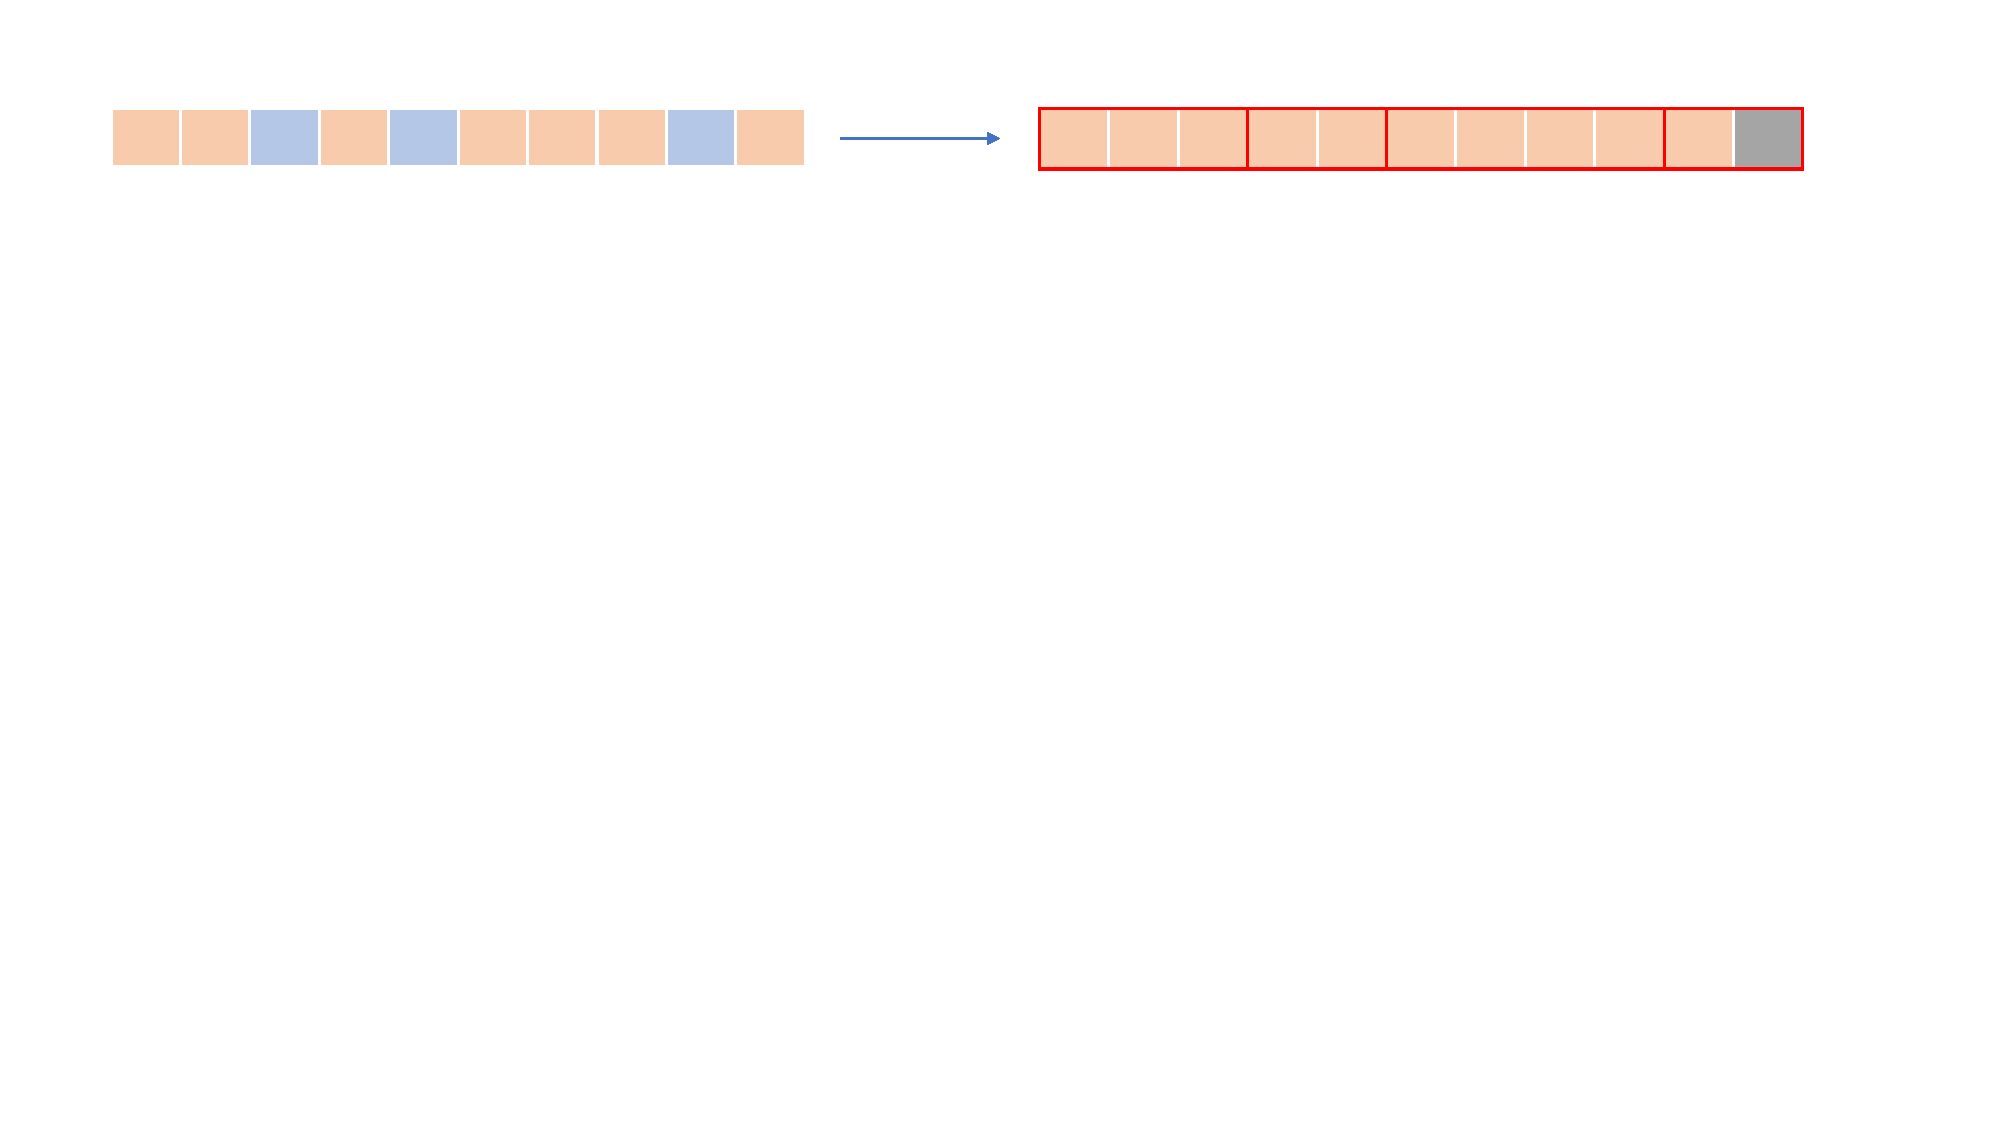
\includegraphics[width = 0.8\textwidth]{./images/dummy_seat.pdf}
        \caption{Problem Conversion with One Seat as Social Distancing}
    \end{figure}
    \end{frame}

  \begin{frame}{Basic Concepts}
    \begin{itemize}
      \item Pattern refers to the seat planning for one row.
      \item A descending form $P_{k} = (t_1, t_2, \ldots, t_n)$ to denote pattern $k$, where $t_h$ is the new group size, $h = 1,\ldots, n$.
      \item For each pattern $k$, $\alpha_k, \beta_k$ indicate the number of groups and the left seats, respectively.
      \item Loss for pattern $k$: $\alpha_k \delta + \beta_k - \delta$.
      \item $I_1$: the set of patterns with the minimal loss-- the largest. 
      \item Full patterns: $\beta_k =0$.
      \item[-] Example: $\delta = 1$, $M =4$, $n_i = i+1, i \in \mathcal{M}$, $L = 21$.
      Largest pattern: $(5, 5, 5, 5), (5, 4, 4, 4, 4), (5, 5, 5, 3, 3)$.
      Full pattern: $(5, 5, 5, 5)$. 
    \end{itemize}
  \end{frame}


  \begin{frame}{Loss of The Largest Patterns}
    \begin{itemize}
      \item[-] A largest pattern can be obtained by the greedy way: select the maximal group size, $n_{M}$, as many times as possible, then $L = n_{M} \cdot q + r, 0 \leq r < n_{M}$, $r$ is the number of empty seats. 
      \item[-] When $r > \delta$, these seats can be occupied by the group type $(r-\delta)$; when $r \leq \delta$, leave these seats empty.
      \item[*] Loss of the largest patterns: $q \delta -\delta + f(r)$, where $f(r) =0$ if $r > \delta$; $f(r) = r$ if $r \leq \delta$.
      \item[*] For a seat layout, $\{S_1, S_2, \ldots, S_{N}\}$, the minimal total loss: $\sum_{j} (\lfloor \frac{S_j+\delta}{n_{M}} \rfloor -\delta + f((S_j + \delta) \mod n_{M}))$. The maximal number of people assigned: $\sum_{j} (S_j - \lfloor \frac{S_j+\delta}{n_{M}} \rfloor + \delta - f((S_j +\delta)\mod n_{M}))$.
    \end{itemize}
  \end{frame}
  
  \begin{frame}{Dynamic Seat Assignment Problem}
    \centering
    \small
    \begin{itemize}
    \item[-] There is and only one group arrival each period. $T+1$ periods in total.
    \item[-] The probability of an arrival of group type $i$: $p_i$. Value function: $V_{t}(\mathbf{L})$. 
    \item[*] Remaining capacity: $\mathbf{L} = (L^{r}_1, L^{r}_2, \ldots, L^{r}_{N})$.  
    \item[*] The number of remaining seats in row $j$: $L^{r}_{j}$. 
    \end{itemize}

    Dynamic seat assignment can be characterized by DP:
    $$V_{t}(\mathbf{L}) = \mathbb{E}_{i \sim p}\left[\max_{\substack{j \in \mathcal{N}: \\ L_j \geqslant {n}_{i}}}\left\{V_{t+1}\left(\mathbf{L}- n_{i}\mathbf{e}_j^{\intercal} \right)+ i, V_{t+1}(\mathbf{L})\right\}\right], V_{T+1}(\mathbf{L}) = 0.$$
    \small
    \begin{itemize}
      \item[-] DP is computationally complex due to the curse of dimensionality.
      \item[-] We give a seat planning by stochastic programming firstly, then apply stochastic planning policy to make the decision.
    \end{itemize}
\end{frame}
